\documentclass[]{article}
\usepackage{graphicx}
\usepackage{subcaption}
\usepackage{siunitx}
\usepackage{longtable}
\usepackage{tabu}
\usepackage{booktabs}
\usepackage{hyperref}
%opening
\title{Reply to NST reviewers}
\author{Zhou Yong}

\begin{document}

\maketitle

\section{Reviewer 1}
\subsection{Question: Why not show $G_{relative}$ distribution against the reference PMT}
\textit{Original statements: P.7 - Fig.7: I believe it would be preferable to show th plot of $G_{relative}$ with respect one of the reference PMT, which remain untouched during the full set of measurements (if I understand well the procedure).} \newline
\textbf{Answer:}
\begin{enumerate}
	\item Although the two fixed PMTs can be used to calculate the $G_{relative}$ of all tested PMTs, they are not necessarily to be adopted as reference PMTs.  Acctually, they are called monitoring PMT  within our test bench system. As pointed out in the general description of the test bench in Sec. 2 of this article, these two PMTs are mainly used to monitor the LED stability and the overall performance of the test bench system. 
	\item Since a relative method is adopted, any PMT can be used to get a $G_{relative}$ distribution using the same set of testing data. In other words, the $G_{relative}$ is dependent on the selection of reference PMT. However, the selection of reference PMT is mainly determined by the purpose of the test bench user. For the PSD PMT selection, the reference  PMT is the one which has underwent a cosmic ray calibration. The calibration works as follows: 1) the reference PMT was coupled to a prototype detector unit and the MIPs spectrum was recorded at a specific initial voltage 2) then adjust the supply voltage of the reference PMT  to move the MIPs peak to the desired value. In this way, the optimal working voltage of the reference PMT can be determined. Since we can calculate $G_{relative}$ of all other PMTs with respect to this reference PMT and its variation against supplying voltage, the optimal working voltages for all other PMTs can then be determined indirectly. Based on these results, we can select the tubes within a specific gain range.
	\item The above procedure for  PSD PMT selection is actually the application of the testing data obtained using our test bench, which is not the subject of this article, thus it is not described in the article. In this article, the tube with the smallest gain has been chosen as the reference PMT to calculate the $G_{relative}$ distribution because this gives the reader a clearer implication of the variation of the gain of the R4443 tubes.
\end{enumerate}

\subsection{Question: More detalis about the integrating sphere and how it works as a perfect integrator for short light pulses}
\textit{Original statements: P.4 - L.36: Can you provide some more details on the integrating sphere and in particular how it works as a perfect light integrator even for relatively short duration pulse of the order of few tens of ns?}\newline
\textbf{Answer:} \newline
The integrating sphere used is a customized product specifically optimized for out test bench. It has a very small diameter of 5 cm, which is not normally seen in the market. It has one input port for LED, and one output port for fiber bundle (see Fig.~\ref{fig:is_drawing}). Both the ports have a diameter of 14 mm, and are arranged \SI{180}{\degree} against each other. A round diffusing baffle is then mounted in the middle of the sphere (see Fig.~\ref{fig:baffle}). The baffle has a slightly larger diameter of 16 mm, just sufficient to cover the two ports. The inner surface of the integrating sphere and the round baffle are both coated with white highly reflective material ($BaSO_4$, \SI{98}{\percent} at 400 nm). The direct light from LED will be blocked by the baffle and reflected back, and all the light will undergo multiple diffusing reflection before reaching the output port. In this way, an uniform and isotropic distribution can be obtained at the output port.

The above deduction is generally true when the integrating sphere works in steady state, i.e. the input light intensity is constant in a relatively long time. For short light pulses, the temporal response of the integrating sphere needs to be considered, which is of the exponential form. The time constant is approximately 5.5 ns for a 5 cm integrating sphere (see \href{http://www.sciencedirect.com/science/article/pii/S016890021500426X/pdfft?md5=6c1ff96a0c12fd90667d756f698abbfc&pid=1-s2.0-S016890021500426X-main.pdf} {Test of candidate light distributors for the muon laser calibration system, NIM A, vol. 788, pp. 43–48, Jul. 2015}). Thus, a light pulse width of several tens of ns is relative long for our integrating sphere and the uniformity in the output port can still be maintained. More importantly, our measurements have confirmed this idea using a 30 ns light pulse.
The result is shown in Fig.~\ref{fig:uniformity_integrationsphere} and the uniformity is within $\pm\SI{0.5}{\percent}$. This degree of uniformity is sufficient for the test bench.


\begin{figure}[!htb]
	\begin{subfigure}[t]{75mm}
		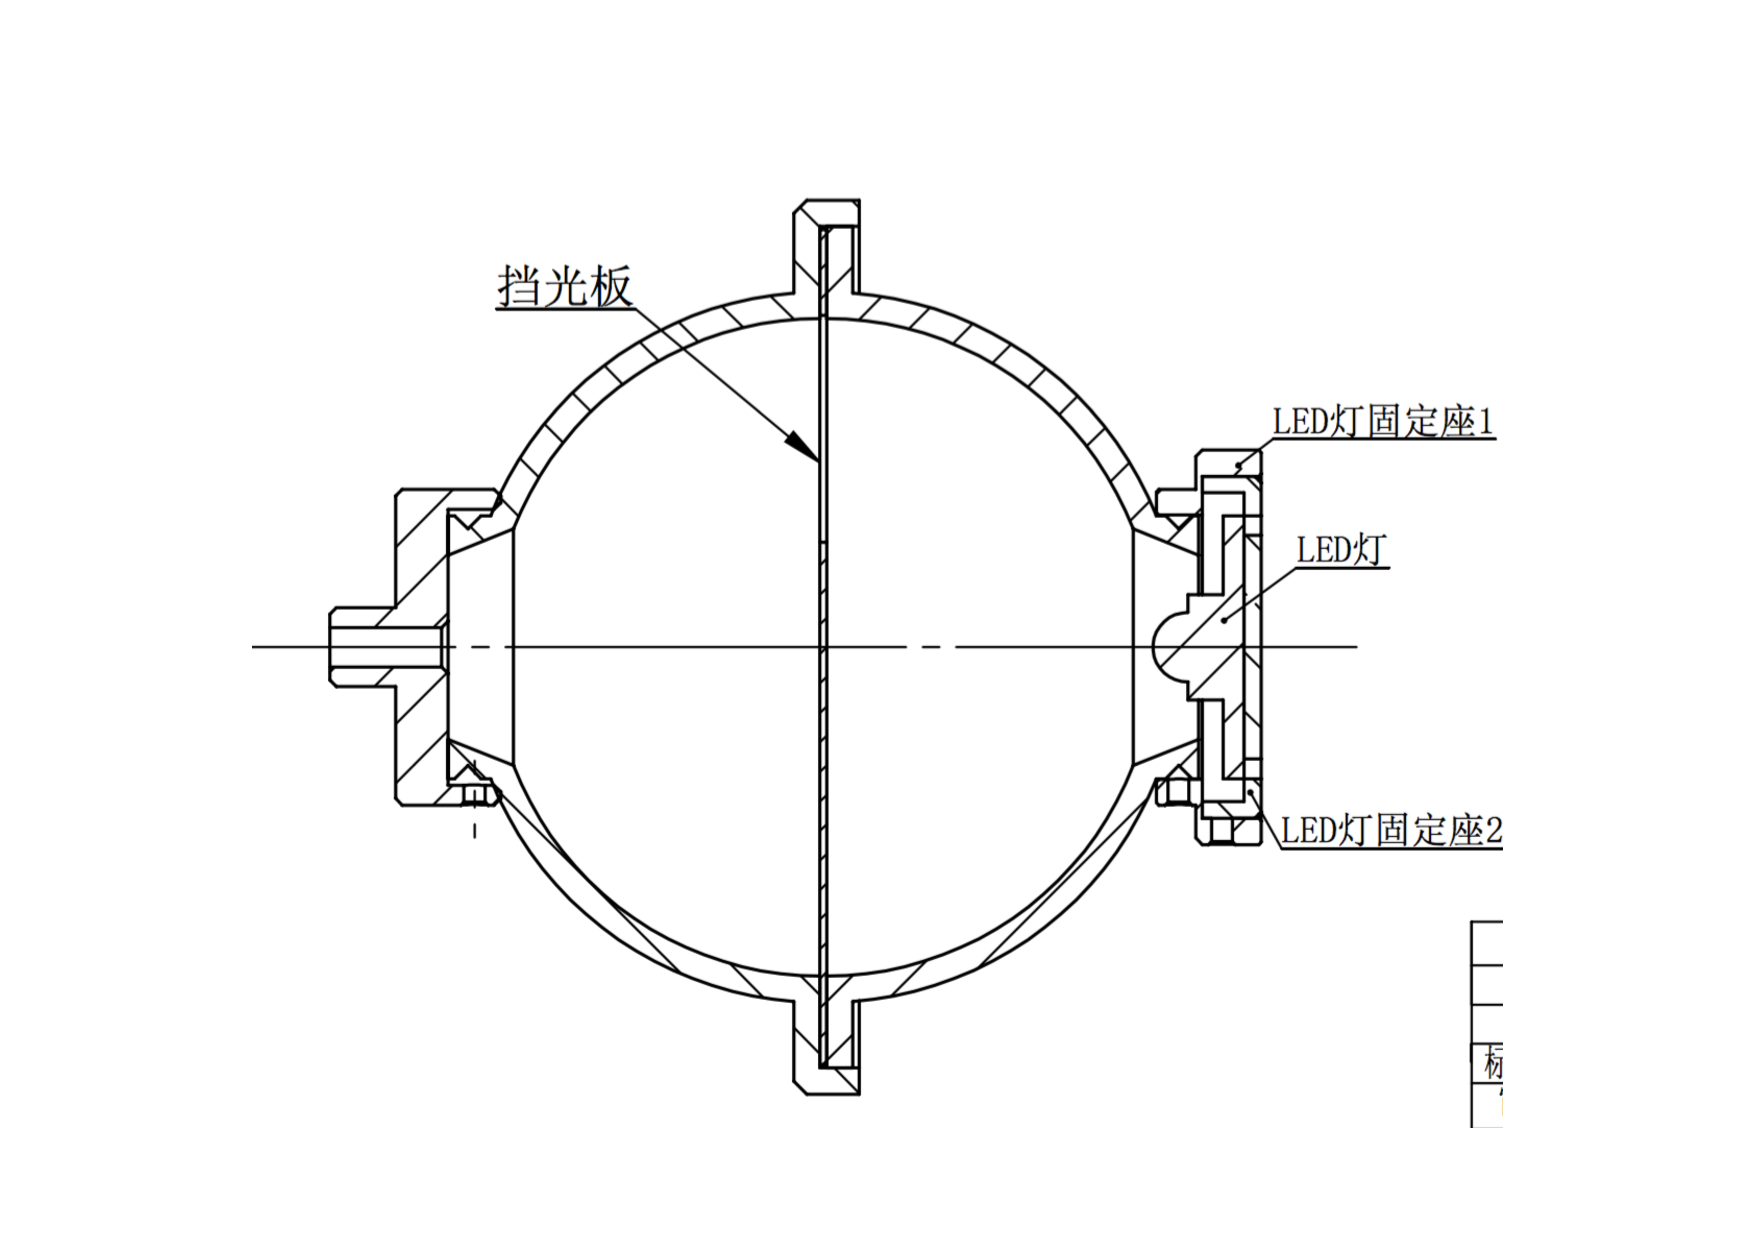
\includegraphics[width=75mm]{is_drawing}
		\caption{Drawing of the 5 cm integrating sphere.}
		\label{fig:is_drawing}
	\end{subfigure}
	\begin{subfigure}[t]{45mm}
		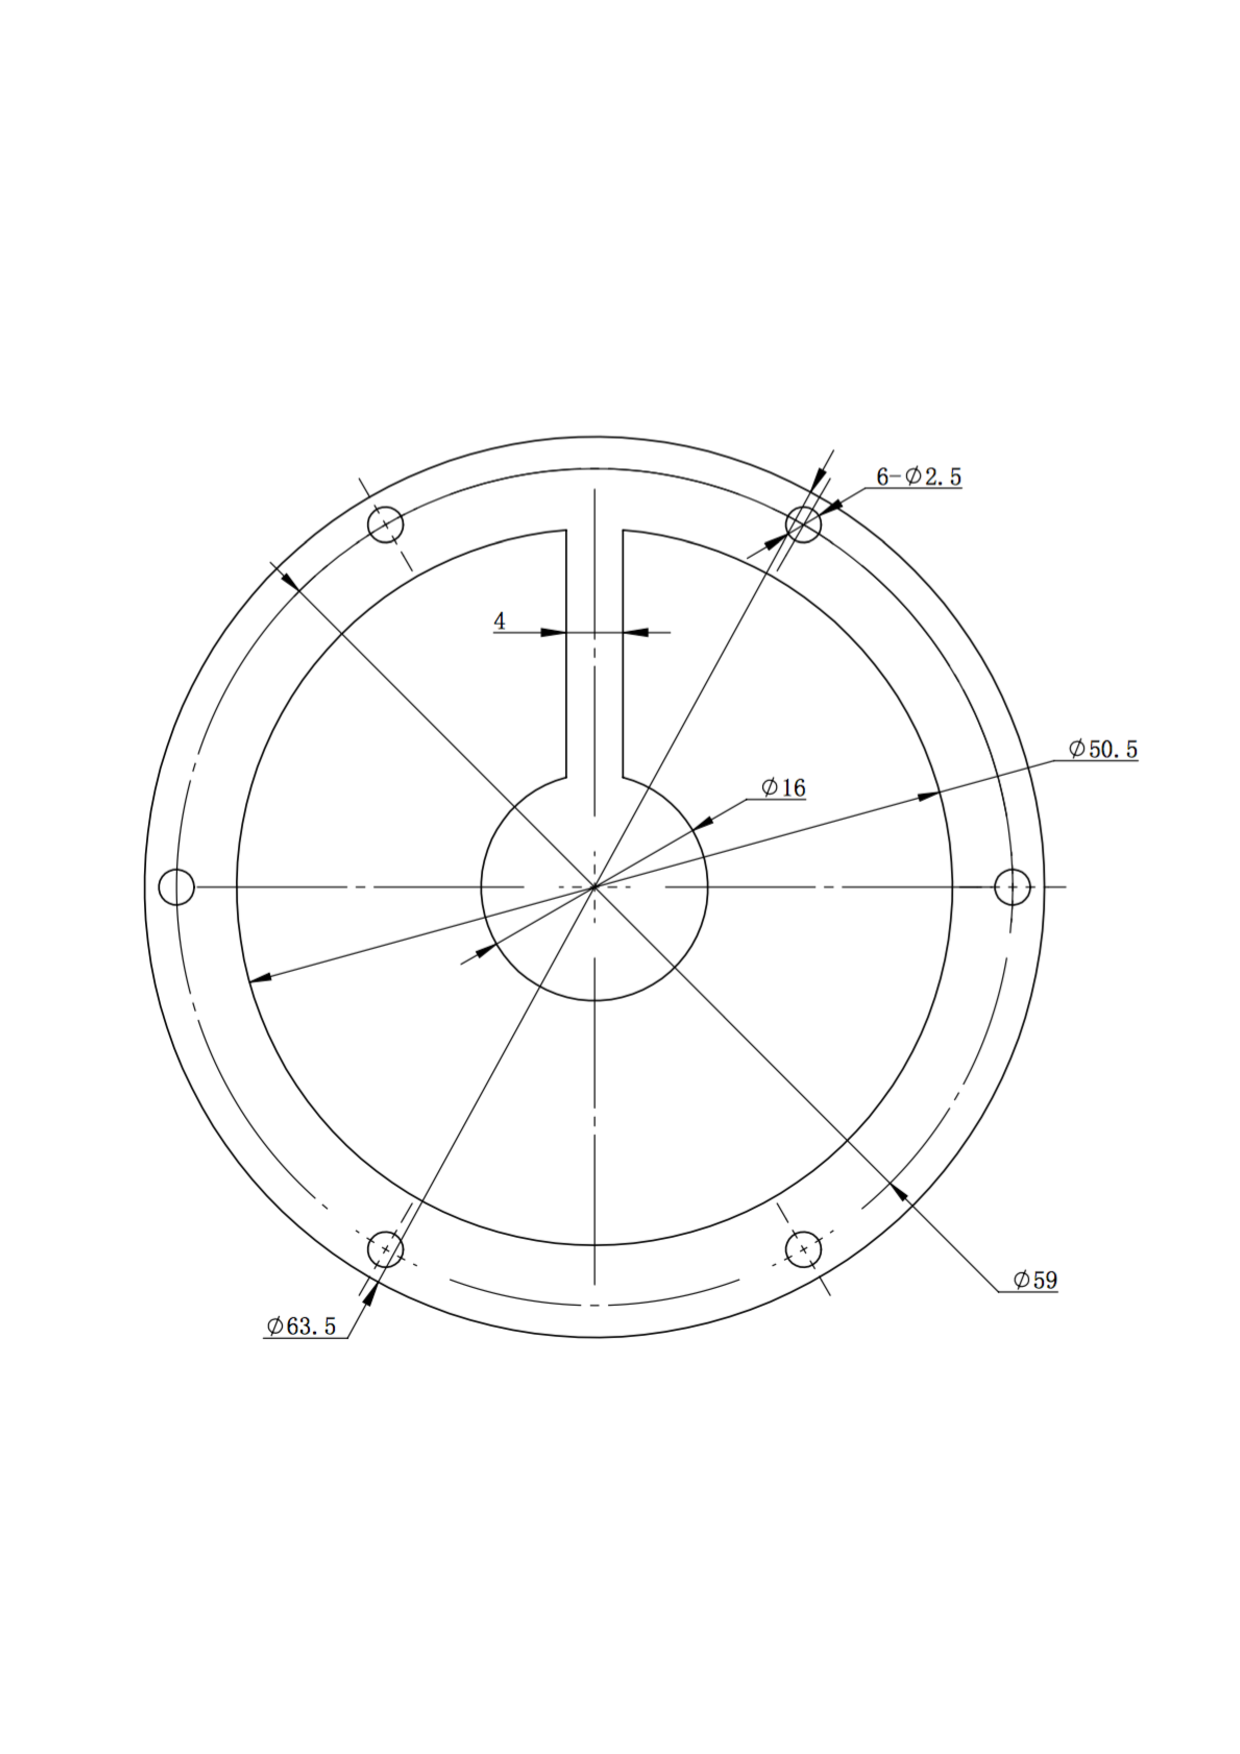
\includegraphics[width=45mm]{baffle}
		\caption{Baffle of the 5 cm integrating sphere.}
		\label{fig:baffle}
	\end{subfigure}
	\caption{Integrating sphere used in the test bench.}
	%\label{fig:FIG2}
\end{figure}

\begin{figure}[!h]
\centering
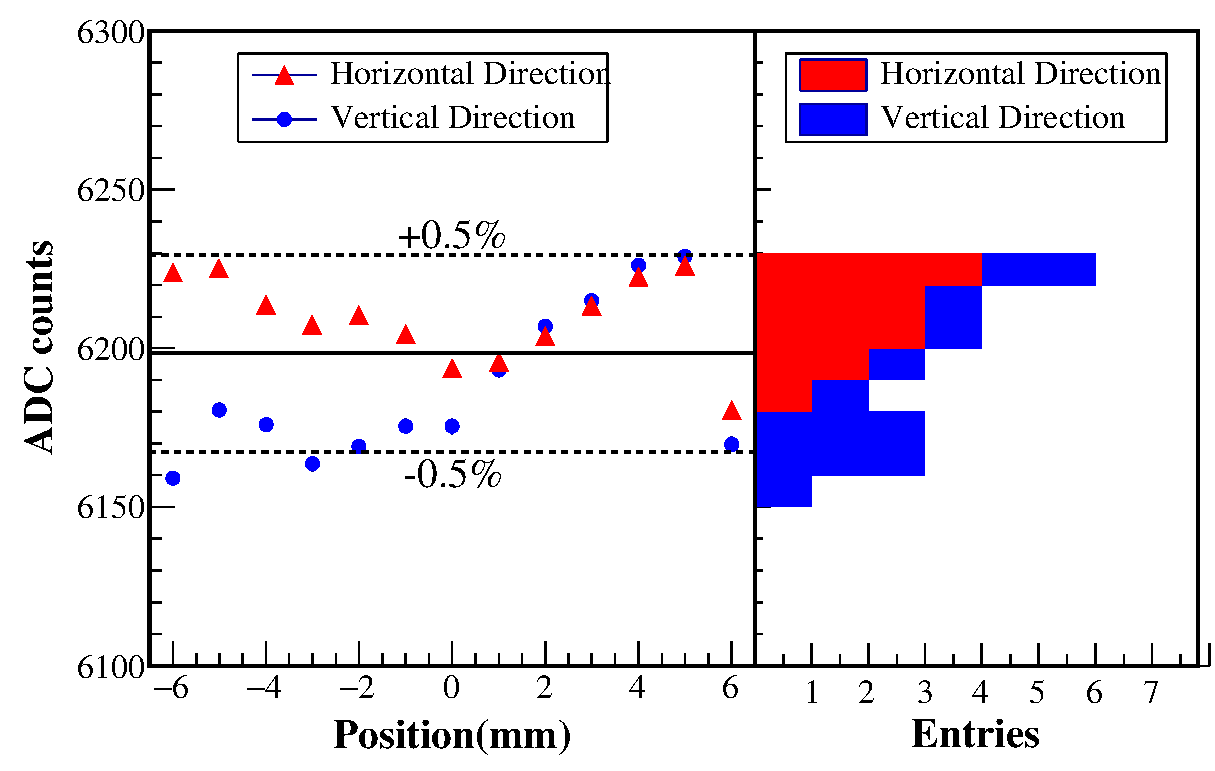
\includegraphics[width=0.7\linewidth]{uniformity_integrationsphere}
\caption{Uniformity of the integrating sphere}
\label{fig:uniformity_integrationsphere}
\end{figure}

\subsection{Question: More infos about R4443}
\textit{Original statements: The paper refers to the Hamamatsu R4443 photomultiplier that however is not listed in the Hamamatsu catalogue and surfing the web I did not find a data sheet for it. If, as I believe to understand, the R4443 is a modified version of the R647 it should be clearly stated and the differences highlighted.}\newline

\textbf{Answer:}\newline
The R4443 tube is actually a ruggedized version of the R647 tube. It has been designed specifically for space usage and is not listed in the general Hamamatsu catalogue. The PSD project adopts the R4443 tube because of its successful usage in the GLAST/FERMI project. You can find the specifications of the R4443 tube used in the PSD detector in the attached datasheet. The datasheet is provided by  Hamamatsu and can't be found in the Internet. 

\section{Reviewer 2}
\subsection{Question: About the bending of the fibers and its effects?}
\textit{Original statement: Do the fiber transmission difference have something to do with the bending of fibers?
Will this degree of bending change during a certain characterization?}\newline

\textbf{Answer:}\newline
It's true that the bending of fiber affects the fiber's light transmission coefficiency. However, the key point for our testing method is the stability of the fiber configuration so that the relative transmission difference between any two fiber channels remain unchanged in a long time. This concern has been taken care of in the design stage and several measures have been taken to keep the fibers stable over time:
\begin{itemize}
	\item The routing of the fibers was carefully chosen so that the bending in any segment of the fibers not exceeding the curvature safety limit proposed by the manufacture. This ensures that all fibers were in good working states.
	\item The ends of the fibers were fixed using stable optical holder made of stainless steel. And customized fiber fixtures were placed at the key points of the fiber routes to confine the fibers' position. In this way, the fibers can't be moved from its confined position without large external force.
	\item The velocity of the stepping motors are limited to a small value so that the mechanical disturbance will not affect the fibers' position.
\end{itemize}

\subsection{Question: More explanation about PSD's working mechanism}
\textbf{Answer:}\newline


\section{Reviewer3}
Original statements:
\begin{enumerate}
	\item Check the references, some mistakes here and there
	\item Summary should be more elaborative
	\item Change the black background of Fig.3(a)
\end{enumerate}
\end{document}
